
Successful operation of modern networked computer systems are not by coincidence or luck.
Network operators heavily relies on the realistic and scalable testing platforms to
evaluate the functionality and the performance of their communication infrastructures and protocols.
Moreover, as the successfully and widely deployed computer networking technology gets deeply integrated into people's everyday lives,
it is no longer optional to protect network against cyber-attacks.
Occurred attacks should be thoroughly studied and its defense carefully implemented to ensure safe and trusted communication of information.
Replaying the attacks happened in real world and, more importantly, practicing, as well as evaluating, the countermeasures become 
enormously difficult if without a virtually simulated or emulated testbed.
Meanwhile, the network today in many domains and settings, are evolving toward the software-defined networking (SDN) paradigm.
SDN promises centralized and rapid network provisioning, holistic management, low operational cost, and improved network visibility.
Multiple SDN simulation and emulation platforms have help expedite the adoption of many emerging SDN-based applications to production systems.
However, all of those virtual simulation or emulation testbeds are highly coupled with the underlying available physical hardware resources.
As the result, their correctness will be corrupted, their scalability limited, and their fidelity compromised,
especially exposed under the common large-scale network settings.
Under the centre theme of securing SDN-enabled large-scale network using high-fidelity and scalable testing system, our research work has four streams.

\Section{Virtual Time Support for Network Emulation}
\label{VT:Sec:Intro}

Linux-container-based network emulation (LCNE) combines many desired features of software simulators and physical testbeds.
Therefore, we first ask not what LCNE can do for computer network, but ask what we can do for LCNE.
Specifically, we address one of the key issues of this attractive methodology.
An ordinary Linux-container-based SDN emulator uses the system clock across all the containers even if a container is not being scheduled to run.
This leads to the issue of both performance and temporal fidelity, especially when handling high workloads during emulation.

Our approach is to develop the notion of virtual time inside containers to improve fidelity and scalability of the container-based network emulation.
A key insight is to trade time for system resources by precisely scaling the system's capacity to match behaviors of the target network.
The idea of virtual time has been explored in the form of time-dilation-based~\cite{ToInfinityBeyond} and
VM-scheduling-based~\cite{VirtTimeOpenVZ, SliceTime} designs, and has been applied to various virtualization platforms including Xen~\cite{DieCast},
OpenVZ~\cite{VirtTimeOpenVZ}, and Linux Container~\cite{TimeKeeper}.
In this work, we take a time-dilation-based approach to build a lightweight virtual time system in Linux container,
and have integrated the system to Mininet~\cite{Mininet} for scalability and fidelity enhancement.
The time dilation factor (TDF) is defined as the ratio between the rate at which wall-clock time has
passed to the emulated host's perception of time~\cite{ToInfinityBeyond}.
A TDF of 10 means that for every ten seconds of real time, applications running in a time-dilated emulated host perceive the time advancement as one second.
This way, a 100 Mbps link is scaled to a 1 Gbps link from the emulated host's viewpoint.
Our system transparently provides the virtual time to processes inside the containers,
while returns the ordinary system time to other processes.
No change is required in applications, and the integration with network emulators is easy (only slight changes in the initialization routine).
The benchmark evaluation and a data center case study demonstrate that, in addition to enhancing Mininet's fidelity and scalability,
our virtual time system is also addresses the synchronization problem in hybrid simulation and emulation.


\section{Introduction}

% Bring in the issues that our approach can address
% Describe them as problems in current simulation/emulation systems
Software defined networking (SDN) centralizes and simplifies control of network management,
and has been increasingly adopted in data centers and internet exchange points~\cite{B4, Meridian, SDX}.
%Software defined networking (SDN) technology separate the network control logic of the network from
%the distributed hardware that implementing the forwarding behaviors.
Similar to traditional computer network systems, it is crucial to perform appropriate testing and evaluation of
SDN-based applications before deploying on a real system.

Researchers in the simulation community have extended various existing network simulators to support SDN capability~\cite{S3F, NS3, OPNET}.
To improve experimental fidelity, researchers have also developed network emulation testbeds
(e.g., Mininet~\cite{Mininet}) that utilize Linux containers over shared hardware resources and
real network stack to run high-fidelity SDN experiments.
However, container-based emulators cannot reproduce the correct behavior of a real network
with a large network topology and high traffic load because of the limited underlying physical resources.
For example, on a commodity machine with 2.98 GHz CPU, 4 GB RAM, and 3 Gbps internal bandwidth,
Mininet can only emulate a network up to 30 hosts, each with a 100 MHz CPU, 100 MB RAM and connected by 100 Mbps links~\cite{ReproNetExprCBE}.
Therefore, increasing SDN testbed scalability and speed without losing the desired fidelity is essential.

% State our idea
In this paper, we present a model abstraction technique to transform an SDN-based network model to a ``one-big-switch'' network model.
The idea was inspired by the work on rule placement optimization in~\cite{OneBigSwitchAbstraction}.
With the highly abstracted network, SDN application developers now only need to consider
simple end-to-end policy when programming a network,
and are shielded from the details on routing policy, switch memory limits,
and distributing rules across switches.
Our work applies the idea of one-big-switch abstraction for enhancing the scalability
of network simulation and emulation, while preserving the end-to-end forwarding logic.

This technique is useful if users only care about the end-to-end behavior rather than
the details within the network, such as hop-by-hop routing, or table lookup on each single switch.

For example, users may want to simulate a large-scale complex network of networks consisting of traditional TCP/IP networks,
SDN networks, industry control communication networks, etc.
The SDN components in this scenario may not be the focus, and thus maintaining only the end-to-end behavior is sufficient for running the hybrid experiment.
Our technique is also useful for real-time network simulation, in which models must be executed
no slower than the wall-clock time in order to interact with real implementations of network protocols and applications.
Failing to do so may result in temporal faults, i.e., the simulation fails to process events before the designated deadlines
required by the emulation or physical components. 
In addition, industrial collaborators may not want to disclose the details of their production network
(e.g., topology, routing, middle-box location and functionality) to modelers for privacy and security concerns.
They can use our model abstraction techniques on the target network and share the resulting ``one-big-switch'' model.
We develop a three-step approach to transform an SDN network to a big OpenFlow switch based network,
while still preserving the network forwarding logic equivalence.
The high-level idea is illustrated in Figure~\ref{OBS:Fig:BigSimOverview},
and the details are discussed in Section~\ref{OBS:Sec:Design}.
We first group all packets into equivalence classes by analyzing the matching fields
(e.g., source/destination MAC address/IP address/port, VLAN id, etc.)
of the OpenFlow rules installed on the switches.
An equivalence class represents a set of packets of the same network forwarding behavior.
We then create a graph-based model for each equivalence class to model its packet forwarding behavior.
Finally, we traverse all the forwarding graph models to generate rules for the big switch,
and the number of rules is largely reduced.
This way, we reduce the SDN network to a big-switch-based network to
improve the scalability of SDN simulation or emulation.

\begin{figure}[t]
\centering
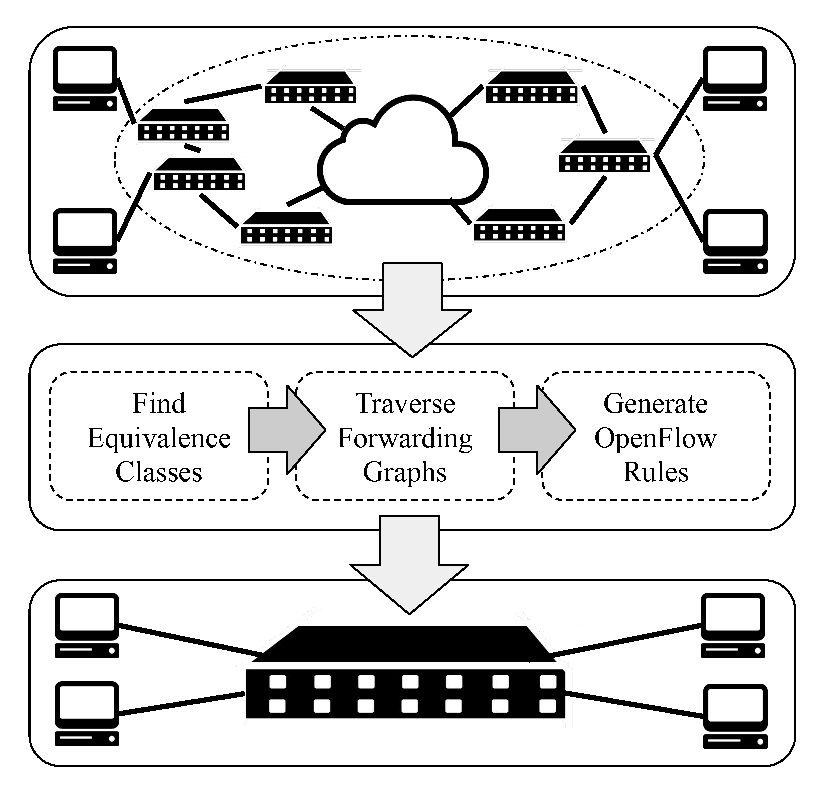
\includegraphics[width=0.9\textwidth]{OneBigSwitch/figures/BigSimOverview.eps}
\caption[One Big Switch Abstraction Overview]{Transforming an SDN network to a
    big OpenFlow switch based network while preserving the network forwarding logic equivalence.}
\label{OBS:Fig:BigSimOverview}
\end{figure}

The reduction in the number of switches and the number of rules significantly enhances the testbed scalability and reduces the experiment running time.
For example, after abstracting a tree-topology network of depth 4 and fanout 3,
the total number of switches required to simulate is reduced from 40 to 1, and the number of rules existed in the SDN network is reduced by 89\%.
The big-switch based network model can save about
75\% to 85\% simulation execution time as compared to simulating the original network.
We can also reuse the abstracted network model.
For example, after one complete experimental run of a complex network,
users can abstract (possibly part of) the network, and reproduce the simulation results with
a much simpler configuration, including link connectivity and flow tables.
We can partition a large-scale network model, and abstract each partition in parallel.
By combining those abstracted network models, a testing platform with limited hardware resources
now can afford such network simulation/emulation experiments.
As the network state evolves, the abstracted big-switch model may also need to be frequently updated.
Our approach is lightweight. For example, we can reduce 50,000+ rules in a large tree-topology network
to 5,000+ rules in a big-switch-based network in three seconds, 
while still preserving the network forwarding rule equivalence.
In addition, our approach allows incrementally updating the big-switch model,
i.e., modifying the rules that are only affected by the current network changes.

In this work, we present a model abstraction technique to reduce networked SDN switches to a one-big-switch model.
We mainly focus on preserving the end-to-end network forwarding logic.
Our long term goal is to investigate systematic model abstraction approaches that preserve end-to-end performance equivalence as well,
such as latency and packet drop, to further enhance the model fidelity.

The remainder of this paper is organized as follows.
Section~\ref{OBS:Sec:MotivatingExample} illustrates the problem and the approach using a simple motivating example.
Section~\ref{OBS:Sec:Design} describes the details of the three-step model abstraction design.
Section~\ref{OBS:Sec:Evaluation} presents the evaluation results in terms of forwarding logic equivalence, simulation time,
reduction in flow rules, and model abstraction execution time.
Section~\ref{OBS:Sec:relatedwork} summarizes the related works, and Section~\ref{OBS:Sec:conclusion} concludes the paper with future works.

\Section{Deep Learning Based Cyber Security System}
\label{DL:Sec:Intro}

Deep learning has gained a dramatic increase in popularity in the last couple of years,
and has offered advanced solutions in the areas of image and speech recognition~\cite{AlexNet, SpeechDNN},
natural language processing~\cite{Word2Vec}, Go playing~\cite{AlphaGo}, and many other domains~\cite{DeepLearning}. 
Motivated by deep learning's success, we ask what deep learning technology can do for cyber security.
Specifically, we focus on the domain of intrusion detection system.
Though both motivated by the deep learning technology, we have different answers for network-based and host-based intrusion detection systems respectively.


\Subsection{Deep Learning Based Network Intrusion Detection System}
\label{DL:SubSec:NIDS}
As networking technology gets deeply integrated into our lives, protecting modern networked systems against cyber-attacks is no longer optional.
Network intrusion detection systems (NIDSes) are essential security solutions for today's networked systems supporting military applications,
social communications, cloud services, and other critical infrastructures.
A NIDS automatically monitors traffic in a network to detect malicious activities and policy violations.
The majority of NIDSes today adopt signature-based detection techniques,
which can only identify known attacks via matching pre-installed signatures to observed network activities. 
The signature databases have to be frequently updated to include new types of attacks.
Those limitations have motivated researchers to investigate anomaly detection based approaches~\cite{STL-NIDS, LOF, RankingOutliner, NB-Tree, RampLossKSVCR, GAA-ADS}. 

Anomaly detection approaches use data mining or machine learning techniques to mathematically model the trustworthy network activities based on a set of training data,
and detect deviations from the model in observed data. A key advantage is the ability to detect unknown or novel malicious activities.
An on-line model further frees network administrators from identifying new patterns or even new types of the abnormal behaviors in a dynamic network environment.
However, if the constructed model is not sufficiently generalized for normal or abnormal traffic,
anomaly-based approaches would suffer from high false positive, i.e., incorrectly treat unknown normal traffic as malicious.

We study the feasibility of off-line deep learning based NIDS by constructing the detection engine with
multiple advanced deep learning models and conducting a quantitative and comparative evaluation of those models.
Specifically, we first introduce the general deep learning methodology and its potential implication on the network intrusion detection problem.
We then review multiple machine learning solutions to two network intrusion detection tasks (NSL-KDD and UNSW-NB15 datasets).
We develop a TensorFlow-based deep learning library, called NetLearner, and implement a handful of cutting-edge deep learning models for NIDS.
Finally, we conduct a quantitative and comparative performance evaluation of those models using NetLearner.


\section{Introduction}
% The harm of malicious software in current days.
While many anti-virus vendors and computer security researchers have fought hard against malicious software for many years,
they remain one of the biggest digital threats in the cyberworld.
Motivated by the high return on investment ratio,
the underground malware industry has been consistently enlarging the sheer volume of the threats on the Internet every year.
According to a report by AV-TEST\cite{AvTest}, the number of total malware by 2018 is estimated at over 800 million,
which has increased 28 times over the past 10 years.
Even worse, recently viciously keen cybercriminals made a lot of efforts to diversify their avenues of attacks\cite{SymantecReport}.
Inspired by the astonishing rise in crypto currency values,
47 new coin mining malware families have emerged since early 2017 and was ascribed to the 956\% soar of the number of crypto mining attacks in the past year~\cite{CryptoMiningAttacks}.
% Similarly, corresponding to the fact that more and more network traffics are coming from mobile devices instead of desktops,
% mobile malware continuous to surge year over year\cite{SymantecReport}.
Traditional signature-based detection approaches have failed to thwart the ever-evolving malware threats.
Therefore efficient, robust and scalable anti-malware solutions are indispensable for protecting the trustworthiness of the modern cyberworld.

% Weakness of existing approaches
A number of recent research efforts\cite{NgramMalwareDetect, QgramMalwareDetect, McBoost, GraphMalwareDetect, YanDataset, AutoEncoderFeatureLearn, AutoEncoderMicrosoft, FunctionCallGraph, YuxinMalwareDnn,NovelFeatureFusion,StaticFeatures,PolySeqCls} have shown that machine learning (ML) offers a promising approach to thwart the voluminous malware attacks.
These efforts have been inspired by the great success of ML in improving the accuracy of image classification, language translation, and many other applications.
There is however a dilemma when we investigate an effective ML-based malware classification system.
On one hand, if we focus too much on finding discriminative malware features to achieve high classification accuracy, the features constructed as such may lose their generality when a different operational environment is encountered.
For instance, although features extracted from the PE headers of malware files have been shown useful in classifying PE malware variants belonging to different families~\cite{yan2013exploring},
a malware classification system trained with these features cannot be used to detect those fileless malware that only exist in the memory.
On the other hand, if the features extracted from malware programs are too generic, such as the frequencies of n-gram byte sequences~\cite{NgramMalwareDetect},
it is difficult to train a malware classifier with high accuracy from them due to their lack of discriminative power~\cite{yan2013exploring}.
%These efforts are inspired by the status quo that ML and DL algorithms have proven high performance in
%image classification, language translation, and many other research fields\cite{DeepLearning}.
% once informative and discriminating features are learned and extracted.
%Still, feature selection makes existing ML- and DL-based detection approaches suffer one or more of the following weaknesses.
%First, people have to spend significant amount of time on, instead of designing smart algorithms, searching non-intuitive and indirect features.
%Secondly, since features are manually picked from a specific dataset, they may not be commonly available in all situations.
%For example, as the most informative part of a binary, PE-header is not always accessible due to varying reasons\cite{YanDataset}.
%Besides, certain golden features are not robust in the face of polymorphic and metamorphic malware.

To strike a balance between generality and performance, we aim to build a malware classification system from malware programs represented as their control flow graphs (CFGs), a data structure commonly used to characterize the control flow of any computer program.
The generality of CFGs for malware classification can be attributed to two factors:
(1) the CFG can be extracted from different formats of malware code, such as binary executable files, exploit code discovered in network traffic~\cite{zhang2007analyzing}, emulated malware~\cite{sharif2009automatic},
and attack code chained together from gadgets in return-oriented programming attacks~\cite{shacham2007geometry},
and (2) the CFG can be used to derive a variety of static analysis features widely used in existing works on ML-based malware classification,
such as n-grams\cite{NgramMalwareDetect}, q-grams\cite{QgramMalwareDetect}, opcodes~\cite{bilar2007opcodes} and structural information~\cite{kong2013discriminant}.
Therefore, a malware classification system trained from CFG-represented malware programs can find applications in various operational environments.

% How CFG and deep learning can help.
%We think the key to overcome these weaknesses is to fully utilize a special kind of representation of executable binary: Control Flow Graph (CFG).In a nutshell,

%A CFG is a directed graph in which the vertices represent a linear sequence of program instructions and the arcs represent execution flow. Taking a global view from a program, it captures the program's control logic because all the possible execution paths are embedded in the graph. Machine learning algorithms can conveniently access such global characteristics via the CFG's adjacency matrix. On the other hand, local semantics of the program is also preserved via the instruction sequences inside the basic code blocks. This leaves us the ability to still selectively extract from vertices features heavily used and proven useful, for example n-grams\cite{NgramMalwareDetect} or q-grams\cite{QgramMalwareDetect}, in previous works. Extracting a vector of pre-defined attributes from each vertex quantifies a plain CFG as an Attributed Control Flow Graph (ACFG) without losing the structural information in CFG. The very first uniqueness of this work is to fully unitize the generic ACFG representation to classify malware families.

Classifying CFG-represented malware programs needs to address two types of performance issues,
classification performance ({\it does the malware classifier achieve high accuracy?}) and execution performance ({\it can the malware classifier work efficiently in practice?}).
As discussed earlier, reducing CFGs to vectors that contain simple aggregate features such as n-grams and opcodes leads to efficient malware classification but usually with poor classification accuracy.
Due to the graph nature of CFGs, previous works have studied use of graph similarity measures to train malware classification models~\cite{hu2009large,cesare2010classification,kong2013discriminant}.
However, some techniques for calculating pairwise graph similarity such as those based on graph matching or isomorphism can be computationally prohibitive,
letting alone that the time needed to compute pairwise graph similarity for a malware dataset scales quadratically with its size.

%and training malware classification models based on pairwise graph similarity data leads to quadratic scalability, making it inappropriate for large malware datasets.

%Before that, however, we still need the final piece of the puzzle: a graph-oriented algorithm capable of distinguishing graphs of different types.
%The graphs are of different number of vertices, generally not organized in order.
%The classification of graph is based on not only the attributes in all the vertices, but also the connection relationship between vertices.
%Previous works rely on pairwise graph similarity to make the call.
%For example, \cite{discovRe} adopted graph matching algorithms (for example, bipartite %graph matching) to tell if two graphs are similar or dissimilar.
%A later work by \cite{GraphEmbedding} start to utilize the embedding concept in deep learning to improve the efficiency of measuring the similarity of the graphs.
%Unfortunately, the scalability of pairwise similarity measurement is fundamentally limited by the quadratic time complexity as the number of graphs increases.
%Additionally, as the definition of similarity is highly depends on applications, works in this track are likely hard to adapt to varying scenarios.

Against this backdrop, in this work we propose to use a state-of-the-art deep learning infrastructure, graph kernel-based deep neural network, to classify malware programs represented as control flow graphs.
Due to their capability of understanding complex graph data, graph kernel-based deep neural network have found success in a number of application domains,
such as protein classification, chemical toxicology prediction, and cancer detection~\cite{ToxicologyPredict, ProteinDataset, SimonovskyEcc, Dgcnn}.
Particularly, our work extends a special type of graph kernel-based deep neural network, Deep Graph Convolutional Neural Network (DGCNN)~\cite{Dgcnn} for classifying CFG-represented malware programs.
Different from graph classification techniques based on pairwise graph similarity,
DGCNN allows attribute information associated with individual vertices to be aggregated quickly through neighborhood defined by the graph structure in breadth-first-search fashion,
thus embedding high-dimensional structural information into vectors that are amenable to efficient classification.

%apply the gradient descent optimization method directly on individual graph samples, which thus alleviates the necessity of embedding graphs into vectors explicitly before the classification step.

%We address the drawbacks of existing graph analysis approaches by introducing the %state-of-the-art deep learning architecture,
%graph kernel based deep neural network.
%It is a good fit for three reasons.
%First, as a set of neural network architectures that predict the class of a graphs on the basis of both graph structure and vertices (and/or edge) features,
%they already achieves fairly competitive performance in domains like protein classification, chemical toxicology prediction, movie collaboration and so on.
%This is attributed to graph kernel based neural network's generalization ability besides its capability to effectively understand the graphic data.
%More specifically we choose to extend the Deep Graph Convolutional Neural Network (DGCNN)\cite{Dgcnn}.
%Unlike the embedding approach\cite{GraphEmbedding} having to train on paired graphs, DGCNN allows end-to-end gradient descent on individual graph samples,
%without the need to first `embed' graph into vectors before classifying.
%Moreover, though our system builds on the existing DGCNN, we have taken a step forward by proposing several modifications to boost its effectiveness.

\if 0
Putting all together, in this paper we present \sysname,
an end-to-end \underline{M}alware detection system characterized by both \underline{A}ttributed control flow \underline{G}raph representation and
us\underline{I}ng deep graph \underline{C}onvolution neural network.
Designed as an data-oriented machine learning pipeline, we illustrate \sysname end-to-end in Figure~\ref{fig:SystemPipeline}.
Starting from the left end, \sysname assumes a raw executable binary is firstly disassembled into intermediate assembly code,
which is readily supported by many binary analysis tools, like IDA-Pro.
Cross-platform assembly code then go through a parser and a extractor that together builds the attributed control flow graph.
System flow ends with a malware prediction made by a pre-trained deep-learning based decision engine,
powered by our carefully re-engineered graph convolution neural network model.
We unveil the design details component by component from Section~\ref{sec:DGCNN} to Section~\ref{sec:Implement}.
\fi

To demonstrate the applicability of DGCNN for malware classification,
we have developed a new system called \sysname (an end-to-end \underline{ma}lware defense system that classifies CF\underline{G}-represented malware programs us\underline{i}ng DG\underline{C}NN).
\sysname improves the effectiveness of malware classification by extending the standard DGCNN with customized techniques tailored for malware classification.
We use two large malware datasets to evaluate the performance of \sysname and the experimental results show that it can classify CFG-represented malware programs with accuracy comparable to those of the state-of-the-art methods applied on handcrafted malware features.
%Experiment result shows MalDenfenser achieves performance comparable to state-of-the-art methods.

The remainder of the paper is organized as follows.
In Section~\ref{sec:System}, we introduce the overall design of \sysname.
In Section~\ref{sec:DGCNN}, we provide a primer on DGCNN and then present our improvements over the standard DGCNN for classifying CFG-represented malware programs.
In Section~\ref{sec:Implement} we discuss a few implementation details of \sysname.
We present our experimental results in Section~\ref{sec:Experiment}.
We discuss related work in Section~\ref{sec:related-work} and draw concluding remarks in Section~\ref{sec:conclusions}.

% In a summary, our contributions made in this work are as follows.
% \begin{itemize}
%     \item First we represent binary executable as the generic ACFG, which not only fully preserves the global semantics of the program,
%     but also extracts highly-customizable attributes of the instruction sequences inside local vertices.
%     \item We start from a state-of-the-art DGCNN to fuse the vertices features according to the graph structure. Our further extensions to the
%     existing neural network provides a certain degree of improvement comparing to the off-the-shelf model.
%     \item Combining the advantages of the ACFG representation and DGCNN, we propose \sysname, an end-to-end malware detection system,
%     and evaluate it with both public and private datasets of significant amount of malware samples.
%     Experiment result shows MalDenfenser achieves performance comparable to state-of-the-art methods.
% \end{itemize}


The remainder of this thesis is structured as follows.
Chapter~\ref{Cpt:RelatedWorks} briefly review the related works for each of the four topics.
Then Chapter~\ref{Cpt:VTS}--~\ref{Cpt:DLMC} discuss aforementioned systems respectively in details,
typically in the order of: introducing motivation, describing system design, providing implementation details if necessary,
then conducting expermimental evaluation, and finally summarizing this stream of work.
Chapter~\ref{Cpt:Conclusion} concludes our entire works.
